\chapter{面向业务问题的受控分析}

\section{分析对象与访问入口}

任务三面向疾病事实和图谱统计，
支持疾病属性、实体关系、知识覆盖、来源构成和类别分布等问题。
正式查询链路由一个统一分析服务承接，
Nexent 任务三智能体和 Web 工作台是该服务的两个调用入口。
Nexent 适合用对话提出问题，工作台适合查看查询计划、结果数据、统计图和成果文件；
两者都经过同一语义规划、只读执行和结果组织流程。
图谱库用于关系子图和来源登记，分析库提供疾病事实表与统计查询；
统一分析服务把分析库返回的证据、图表和来源范围组织到同一分析结果中。

任务三的实现流程见图~\ref{fig:task3-pipeline}。
系统先把问题转换为一个或多个查询计划，
再执行安全检查和只读查询，
最后形成一条可复用的分析结果记录。

\begin{figure}[H]
\centering
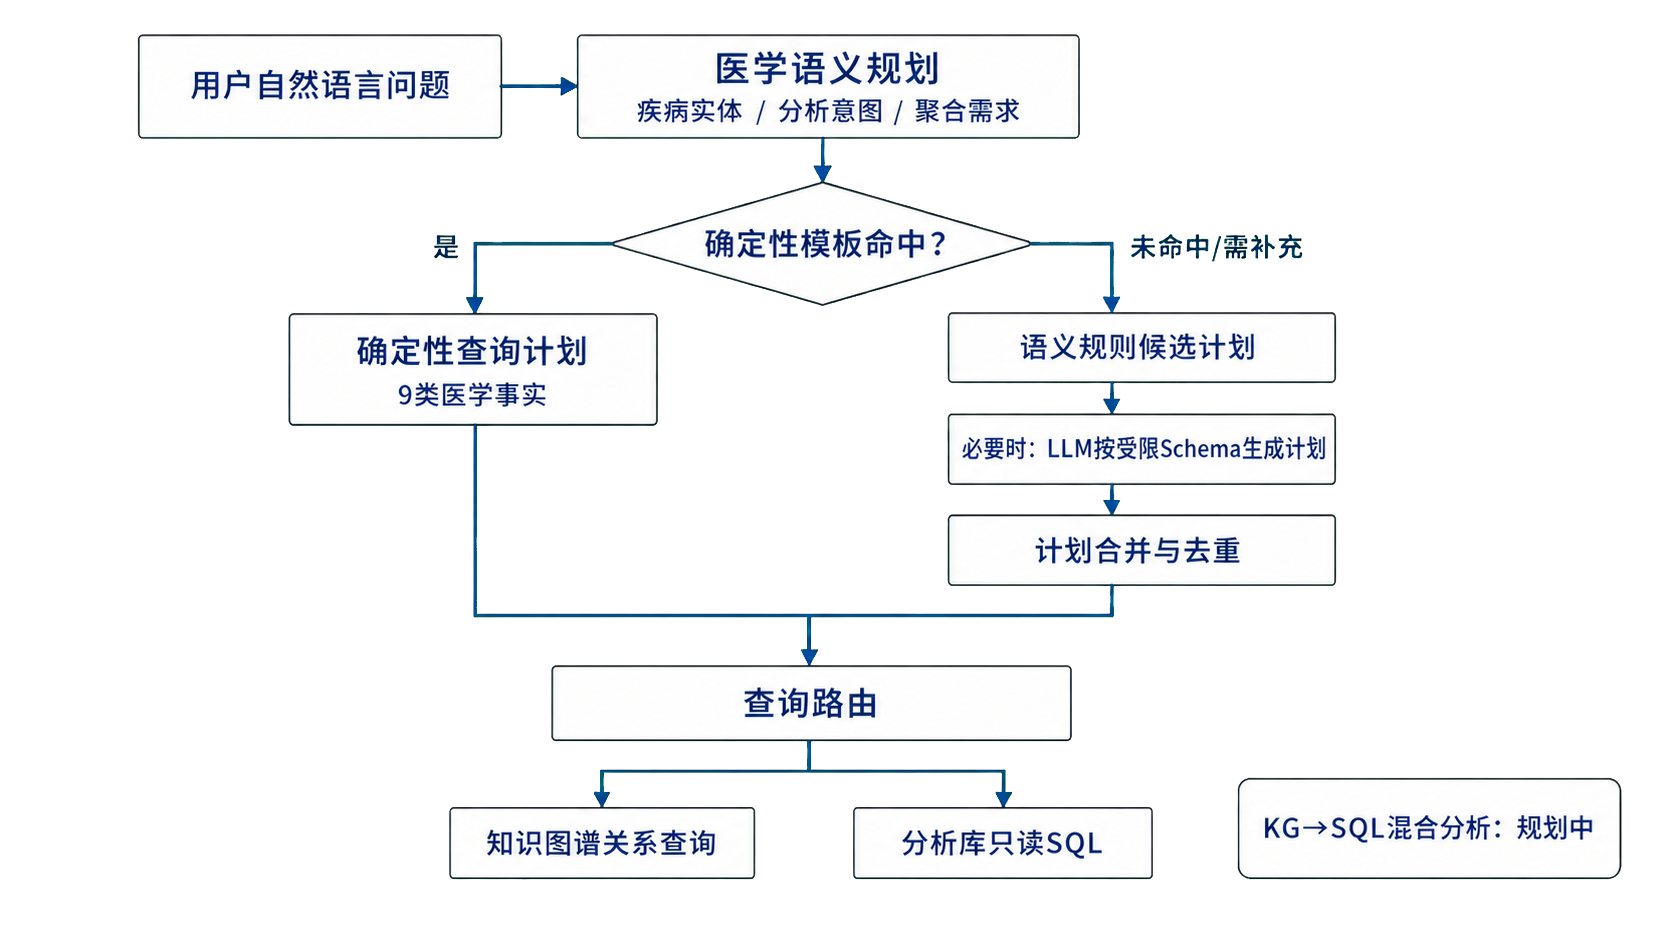
\includegraphics[width=0.90\textwidth]{figures/task3-planning.png}
\caption{任务三的语义规划与查询路由}
\label{fig:task3-pipeline}
\end{figure}

图~\ref{fig:task3-pipeline}把任务三的规划阶段拆成两条受控分支：
命中确定性模板时生成九类医疗事实查询计划，
未命中模板时先由语义层生成候选计划；
只有在语义层判定仍需补充且模型服务可用时，
才请求模型按 Schema 约束生成候选计划，
然后按 SQL 和数据源去重并限制查询数量。
任务三智能体在工具路由阶段再按问题类型选择知识图谱关系查询或统一只读 SQL 分析。
模型服务未配置或调用失败时，系统保留可验证的语义层结果并标记降级，
不会把模型未返回的内容当作查询结果。
图右下角的“KG$\rightarrow$SQL 混合分析：规划中”是后续扩展方向，
不属于当前实现，也不计入本报告的评测结果。

\section{基于语义规划的查询路由}

医疗语义层将自然语言中的疾病名称和关系意图映射到实际业务表。
系统从疾病主表中匹配名称，
当多个疾病名同时出现时优先采用更长、更具体的名称。
症状、药物、并发症、科室、检查、治疗、易感人群、病因和预防
分别对应 9 个事实定义，
每个定义明确目标表、疾病字段、结果字段、显示标题和默认排序。

“某病有哪些症状”“某病应该做哪些检查”等问题直接生成受控查询；
实体类型分布、关系类型分布和科室疾病分布使用预置统计视图。
对于包含多个条件或未命中模板的问题，
语义层先生成可验证的候选计划；
当问题仍需要开放式补充且模型服务可用时，
规划器才请求模型返回受限 JSON 查询计划，
并将模型计划与已识别的语义计划按 SQL 和数据源去重，
最终保留最多 4 项查询。
这套顺序使常用业务问题采用稳定模板，
复杂表达仍可扩展到受控查询；当模型服务不可用时，结果会明确标记为降级。

任务三智能体先判断用户要求的是疾病事实、图谱关系、数据来源还是统计分析，
再由任务级工具选择对应的只读能力。
疾病详情、统计、排名和解释类自然语言问题统一调用
\texttt{ask\_medical\_analytics}，进入同一个语义规划器和分析服务；
常见问题使用确定性模板，复杂问题再使用结构化查询计划。
关系子图和来源清单仍由专用工具直接读取对应的图谱表，
图谱关系查询与统计分析结果使用各自独立的结果口径。
因此，Nexent 的对话分析和工作台的可视化结果都遵循同一结果对象契约，
不会在两个入口各自维护一套自然语言查询执行逻辑。

代码上，\path{task3/runtime.py} 是服务装配入口。
Web 工作台通过 \path{analysis_runtime.py} 调用它，
MCP 通过 \path{mcp_server/tools/task3_runtime.py} 调用它。
\path{execute_nl2sql} 保留为兼容旧智能体配置的工具名，
但与 \path{ask_medical_analytics} 使用同一个服务实例、同一分析库和同一结果契约。
\path{query_disease_analytics} 只保留旧调用方所需的结构化字段投影，
不再作为任务三智能体的自然语言主路由。

智能体不会直接修改分析库。
涉及数据接入、重新建图或刷新来源的请求，
先进入任务二建图工具；
涉及查询的请求只能生成单条\texttt{SELECT}或\texttt{WITH}语句，
并由服务端执行表名、只读连接、时限和返回行数检查。
查询失败、数据不足或问题超出当前表结构时，
分析结果记录保存相应状态和口径说明，
回答只引用实际返回的数据。

\section{自然语言查询的只读执行}

查询安全模块要求 SQL 以 \texttt{SELECT} 或 \texttt{WITH} 开头，
并且只能包含一条语句。
注释、数据库附加、结构修改和数据写入关键字在执行前被拦截，
表名必须位于 17 个允许查询对象（14 张表和 3 个视图）的清单中。
SQLite 通过 URI 只读模式打开，
连接后再设置 \texttt{PRAGMA query\_only=ON}。

执行器为每项查询安装 5 秒进度中止条件，
最多返回 200 行；
一次分析最多执行 4 项查询。
每项结果保存标题、SQL、参数、列、数据行、返回数量和耗时，
单项查询的状态互相独立。
这些限制同时应用于语义模板和模型生成计划，
并由统一分析服务对两个调用入口执行。

\section{分析结果呈现}

分析服务根据查询标题与数据列组织文字回答，
原始返回行同步保留为结果表。
图表策略先读取用户是否明确要求图形，
再根据维度类型和记录数量选择展示形式。
时间字段才允许使用折线图；
类别比较使用条形图或柱状图；
构成比例使用环形图，并保留前 8 类、其余合并为“其他”。
条形图最多展示 20 类，柱状图最多 12 类，折线图最多 16 个点。

分析结果记录包含以下内容：

\begin{itemize}
  \item 用户问题、识别主题和查询计划；
  \item 每项查询的 SQL、参数、列和数据行；
  \item 文字回答、结果说明和数据口径；
  \item 图表类型、标题、维度字段、数值字段和截取规则；
  \item 分析标识、数据库文件名、查询数量、返回行数和执行耗时。
\end{itemize}

每次分析生成独立分析标识。
页面中的回答、结果表和统计图都读取同一对象，
导出模块也按该标识取得当前结果，
使屏幕展示与下载文件使用相同的数据行。
图~\ref{fig:task3-result-object} 展示从问题识别、查询计划到分析结果记录的具体映射。

\begin{figure}[H]
\centering
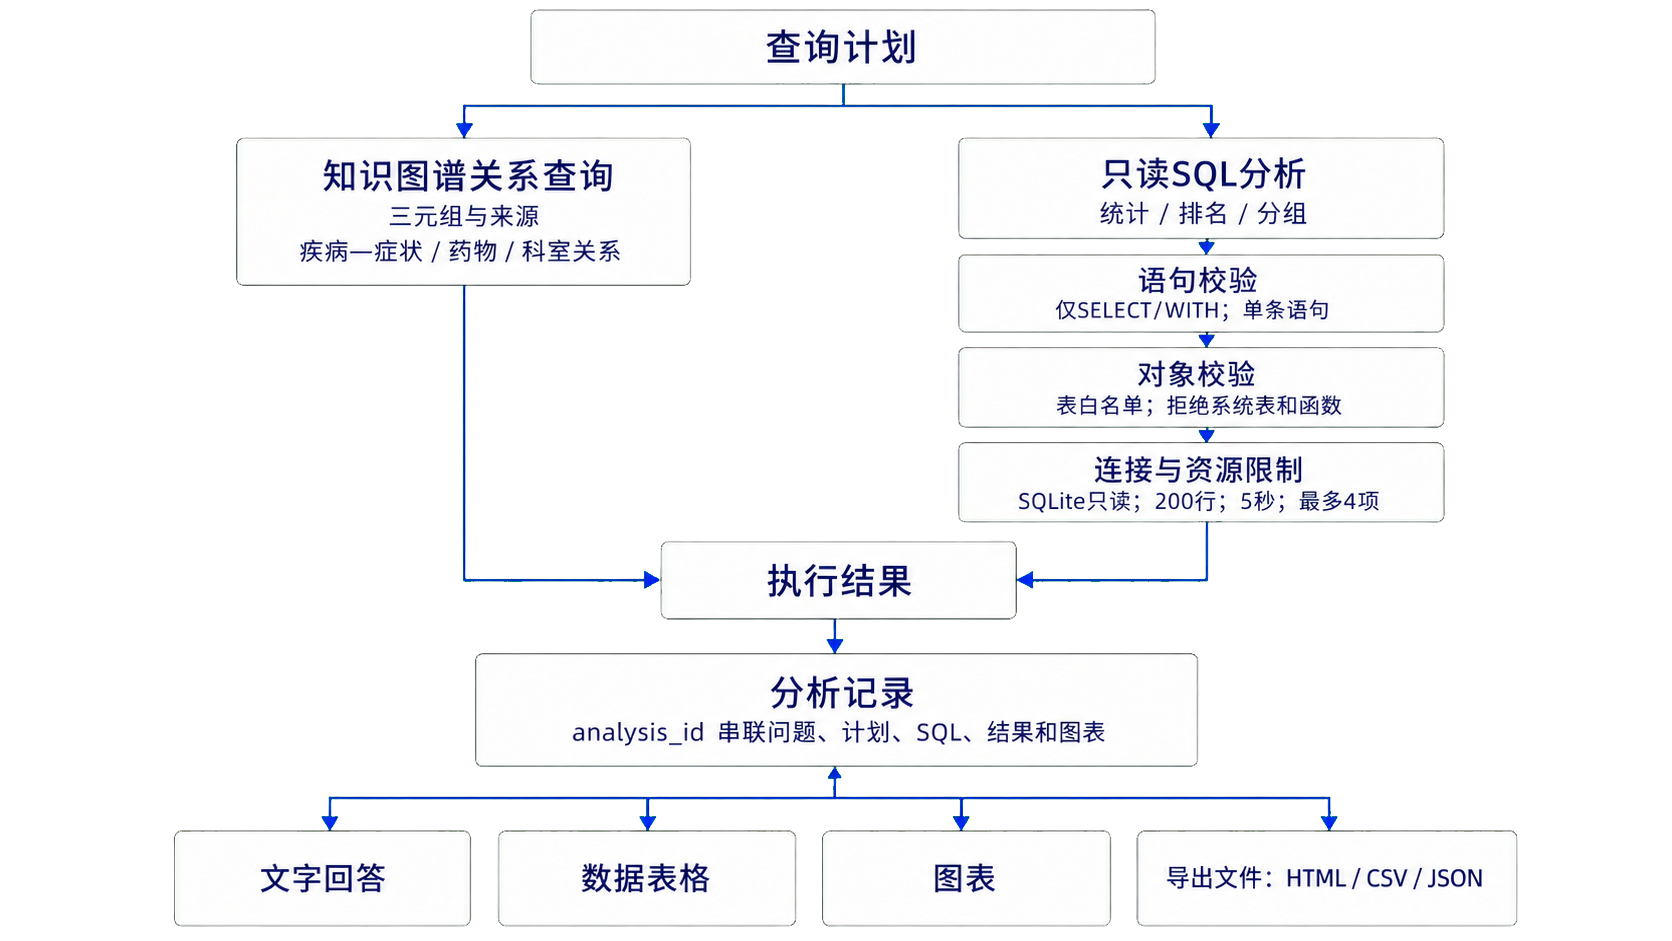
\includegraphics[width=0.90\textwidth]{figures/task3-execution-delivery.png}
\caption{任务三的受控执行与统一结果交付}
\label{fig:task3-result-object}
\end{figure}

图~\ref{fig:task3-result-object}说明两个查询分支如何汇入同一执行结果：
图谱关系查询工具面向疾病、症状、药物和科室关系，
统一分析服务面向疾病详情、统计、排名和分组问题；
SQL 分支依次通过语句、对象、连接和资源检查，
最后由同一分析记录驱动文字回答、数据表、图表和 HTML、CSV、JSON 导出。

图谱库与分析库承担不同职责，不能把两者的数量混写：
图谱库保存规范化实体、三元组和来源，
分析库保存由这些事实投影得到的疾病事实表和统计视图。
因此，图中的“图谱关系查询”不表示统计 SQL 直接读取三元组表；
统计、排名和分组问题仍在分析库上执行只读 SQL，
具体数量以同一运行核验快照中的数据表为准。

\section{知识图谱的关系浏览}

关系图直接读取图谱中的实体和三元组。
用户选择疾病后，
系统按症状、药物、检查、科室、治疗和并发症等关系展开相邻节点。
节点样式和图例在在线界面中区分实体类型，
节点数较多时按关系类型与数量限制展开。
导出的数据表以实体名称、关系名称、分组可靠性分和来源字段保存图中事实。
对任务二增量写入的关系，来源字段包含数据集、文件名、记录号和原文证据；
用户可以从图上的一条边回到任务一最终数据集中的具体文件与记录。

图谱浏览与统计分析可以在同一工作台切换。
关系图适合查看具体疾病的知识结构，
统计图适合比较实体类型、关系类型和来源贡献。
两种展示由同一工作台组织：关系图读取图谱库，统计图读取分析库；
用户能够从总体分布继续查看具体事实。

\section{分析成果导出}

报告模块从当前分析结果记录生成压缩包，
其中包含 HTML 报告、按查询拆分的 CSV 数据和“分析追溯”JSON。
HTML 保存问题、回答、查询步骤、结果表和图表说明；
每项查询单独生成 CSV；
JSON 保存分析计划、SQL、执行状态、来源和完整结果结构。
导出入口按分析标识读取页面已经展示的数据；
当标识对应的结果记录不可用时，服务返回状态信息，要求重新发起分析，
不会在导出阶段静默替换原结果。

HTML 适合离线阅读与成果交流，
CSV 可继续进入统计工具，
分析追溯 JSON 用于保存完整结果结构和接口联调。
